% Define the subtitle of the page
\title{Getting Started}

% Begin the content of the page
\subsection{Getting Started}
Getting started with Edward is easy. 

\subsubsection{Quick Installation}
To install the latest stable version, run

\begin{lstlisting}[language=Java]
pip install edward
\end{lstlisting}

To install the latest development version, run

\begin{lstlisting}[language=Java]
pip install -e "git+https://github.com/blei-lab/edward.git#egg=edward"
\end{lstlisting}

See the \href{troubleshooting.html}{troubleshooting page} for detailed
installation instructions.


\subsubsection{Your first Edward program}

Let's use Edward to fit a simple Bayesian neural network regression model.

First, import Edward, TensorFlow, and Numpy.
\begin{lstlisting}[language=Python]
import edward as ed
import tensorflow as tf
import numpy as np  
\end{lstlisting}

Now, consider the likelihood of an observation $(y_n, x_n)$
\begin{align*}
  p(y_n \mid \mathbf{z} \;;\; x_n, \sigma^2)
  &=
  \mathcal{N}(y_n \;;\; \mu(x_n\;;\;\mathbf{z}), \sigma^2)
\end{align*} 
where $\mu$ is a neural network with weights (latent) variables 
$\mathbf{z}$. Here $x_n$ is the (known) covariate and $\sigma^2$ is the
(known) variance of the observation.

A Bayesian neural network further posits a prior on the weights. Assuming an
independent standard normal prior gives the following joint density
\begin{align*}
  p(\mathbf{z}, \mathbf{y} \;;\; \mathbf{x}, \sigma^2)
  &=
  \mathcal{N}(\mathbf{z} \;;\; \mathbf{0}, I)
  \times
  \prod_{n=1}^N
  \mathcal{N}(y_n \;;\; \mu(x_n\;;\;\mathbf{z}), \sigma^2).
\end{align*}

Here is one way to write this model in Edward. (This is abridged;
full code 
\href
{https://github.com/blei-lab/edward/blob/master/examples/getting_started_example.py}
{HERE}.)

\begin{lstlisting}[language=Python]
class BayesianNN:
    """A Bayesian neural network regression model (abridged)"""

    def log_prob(self, xs, zs):
        # Specify the prior on latent variables zs
        log_prior = tf.reduce_sum(norm.logpdf(zs, loc=0, scale=1), 1)

        # Extract (y,x) from data xs
        y = xs[:, 0]
        x = xs[:, 1:]

        # Specify mu (neural network)
        mus = tf.pack([self.mapping(x, z) for z in tf.unpack(zs)])

        # Specify the likelihood
        log_lik = tf.reduce_sum(norm.logpdf(y, loc=mus, scale=self.lik_variance), 1)

        return log_prior + log_lik
\end{lstlisting}

Instantiating this model as 
\begin{lstlisting}[language=Python]
model = BayesianNN(layer_sizes=[1, 2, 2, 1])
\end{lstlisting}
defines a two-layer a Bayesian neural network regression model with $\tanh$
activation functions. Specifically
\begin{align*}
  h_{11} &= \tanh(w_{11} x_n + b_{11})\\
  h_{12} &= \tanh(w_{12} x_n + b_{12})\\
  h_{21} &= \tanh(w_{211} h_{11} + w_{212} h_{12} + b_{21})\\
  h_{22} &= \tanh(w_{221} h_{11} + w_{222} h_{12} + b_{22})\\
  \mu &= \tanh(w_{31} h_{21} + w_{32} h_{22} + b_3)
\end{align*}
where $\mathbf{z} = (w_{1:}, w_{2::}, w_{3:}, b_{1:}, b_{2:}, b_3)$.

Next, specify a variational approximation to the posterior. A mean-field normal
approximation is reasonable.
\begin{lstlisting}[language=Python]
variational = Variational()
variational.add(Normal(model.num_vars))  
\end{lstlisting}

Finally, simulate a toy dataset of 50 observations with a cosine nonlinearity
and some measurement noise.

\begin{lstlisting}[language=Python]
def build_toy_dataset(n_data=50, noise_std=0.1):
    x = np.linspace(-3, 3, num=n_data)
    y = np.cos(x) 
    y = y + ed.stats.norm.rvs(0, noise_std, size=n_data).reshape((n_data,))
    x = x.reshape((n_data, 1))
    y = y.reshape((n_data, 1))
    data = np.concatenate((y, x), axis=1)
    data = tf.constant(data, dtype=tf.float32)
    return ed.Data(data)  
\end{lstlisting}

Plotting the data shows the relationship between $x$ and $y$.

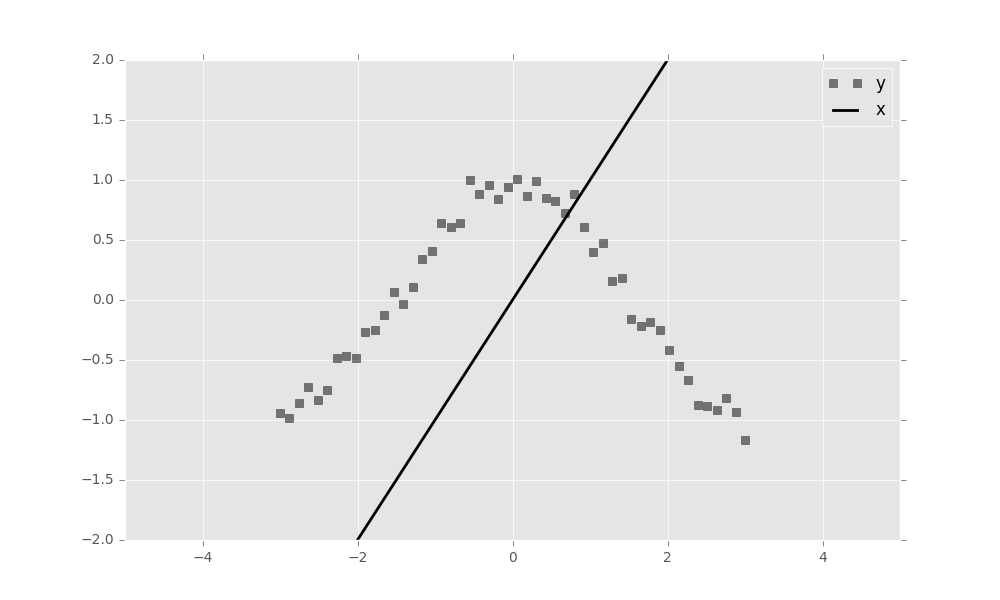
\includegraphics[width=700px]{images/getting-started-fig0.png}

We now have all the ingredients to infer the posterior of this model. 
Edward \texttt{Inference} classes take three things as input: a
probability model, a variational model, and data. Here we run mean-field
variational inference for \texttt{1000} iterations, by subsampling \texttt{5}
datapoints at each
iteration. We also print a status report to the terminal every \texttt{100}
iterations
\begin{lstlisting}[language=Python]
inference = ed.MFVI(model, variational, data)
inference.run(n_iter=1000, n_minibatch=5, n_print=100)  
\end{lstlisting}

Drawing samples from the posterior shows how the Bayesian neural network has
learned the cosine nonlinearity. 

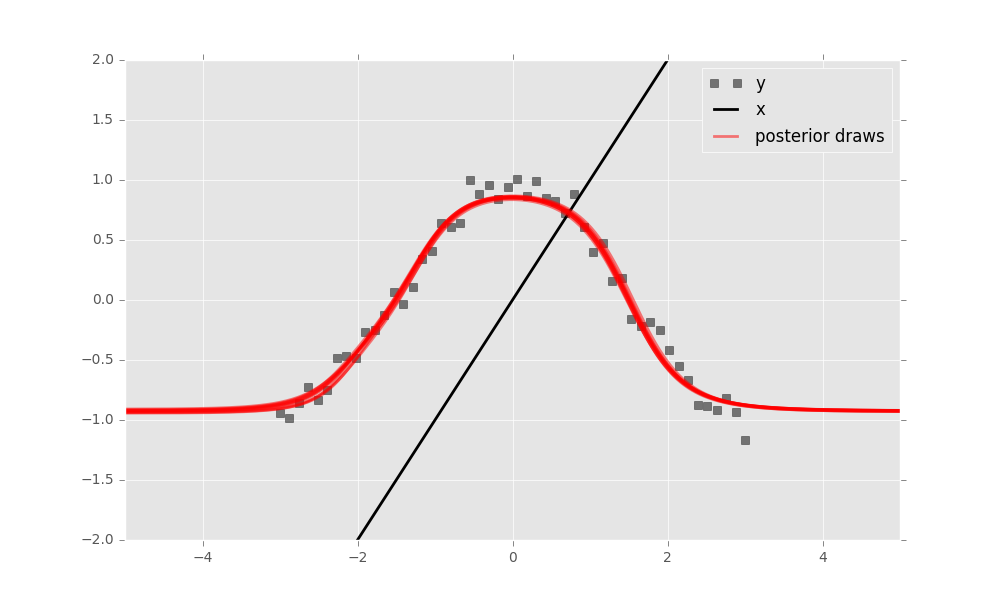
\includegraphics[width=700px]{images/getting-started-fig2.png}

To learn more about Edward, \href{delving-in.html}{delve in}!

If you prefer to learn via examples, then check out our 
\href{tutorials.html}{tutorials}.
